\documentclass[12pt, a4paper]{report}

\usepackage[margin=1in]{geometry}
\usepackage[utf8]{inputenc}
\usepackage[T1]{fontenc}

\usepackage{times}

\usepackage{float}

\usepackage{url} % To put URLs
\usepackage{xurl} % Avoids URLs to overfull \hbox

\usepackage{graphicx}
\graphicspath{{img/}} % Images global configuration
\usepackage[colorlinks=false, pdfborder={0 0 0}]{hyperref}

\usepackage{tabularray}

\usepackage[table, svgnames]{xcolor}
\usepackage{listings} % To use listings

\title{
  Understanding Data Compression: Theory, Techniques, and Modern Tools
}
\author{
  Enrico Marchionni\\
  \texttt{enrico.marchionni@studio.unibo.it}
}
\date{\today}

\usepackage[backend=biber, style=alphabetic, sorting=ydnt]{biblatex}
\addbibresource{references.bib}

\usepackage{amsthm} % To make definitions
\newtheorem{definition}{Definition}[section] % Custom environment for definitions
\newtheorem{example}{Example} % Custom environment for examples

\usepackage{tikz} % For graphs and overlaying text
\usepackage{pgfplots}
\pgfplotsset{compat=1.18}
\usepackage{amsmath} % For math symbols
\usepackage{forest} % For binary trees

\definecolor{C_comment_green}{rgb}{87, 166, 74}
\definecolor{C_keyword_blue}{RGB}{86, 156, 214}
\definecolor{C_macro_purple}{RGB}{199, 120, 221}
\definecolor{C_function_amber}{RGB}{220, 220, 100}

\lstdefinelanguage{CStyle}{
  morekeywords={
    for, while
  },
  morekeywords=[2]{ % macros
    EOF
  },
  morekeywords=[3]{ % functions
    getc, high_range, low_range, output, input_code, find_symbol_straddling_this_range, putc
  },
  sensitive=true,
  morecomment=[l]//,
  morecomment=[s]{/*}{*/},
  morestring=[b]",
  morestring=[b]',
  commentstyle=\color{C_comment_green},
  keywordstyle=\color{C_keyword_blue}\bfseries,
  keywordstyle=[2]\color{C_macro_purple}\bfseries,
  keywordstyle=[3]\color{C_function_amber}\bfseries,
  stringstyle=\color{red},
  identifierstyle=\color{black},
  basicstyle=\ttfamily,
  literate={->}{{\textcolor{black}{->}}}2
            {>=}{{\textcolor{black}{>=}}}2
            {<=}{{\textcolor{black}{<=}}}2
            {!=}{{\textcolor{black}{!=}}}2
            {==}{{\textcolor{black}{==}}}2,
}

\lstset{
  basicstyle=\ttfamily,                 % Set font type
  keywordstyle=\color{blue}\bfseries,   % Set keyword color to blue and bold
  stringstyle=\color{red},              % Set string color to red
  commentstyle=\color{C_comment_green}, % Set comment color to gray and italic
  breaklines=true,                      % Enable line breaking
  frame=single,                         % Add a frame around the code
  numbers=left,                         % Add line numbers on the left
  numberstyle=\tiny\color{gray},        % Style for line numbers
  backgroundcolor=\color{lightgray!20}, % Background color
  captionpos=b,                         % Caption position at the bottom
  showstringspaces=false                % Don't show spaces in strings
}

\usepackage{lastpage} % To keep track of the total number of pages
\usepackage{fancyhdr} % To define custom page numbering

\begin{document}

\maketitle

\begin{abstract}

Data compression is intended as the practice of reducing the size of binary digital data.
It could be considered as a procedure that takes a bit-stream in input and returns another bit-stream as output.
The result may be of equal length or hopefully shorter than the original.

The crucial point to understand data compression is to discuss the distinction between data and information.
It can be said that data is how information is represented\footnote{Ex. the number 0 can be expressed in binary as a sequence of a
certain number of zeros, from \(1\) to \(\infty\), and we know that calculators use at least 8 bits, let's say \(n\)
(considering it as a multiple of 8), to represent an integer number. So at the end \(n - 1\) bits are redundant in the 0
representation on a calculator.}.
In simple terms, data can be compressed because its original representation is not the shortest possible.
The goal of data compression is to reduce data redundancy by maintaining the same amount of information.

The counterpart is that in our time data is inherently redundant, enabling applications to handle various formats.
So data compression isn't only a procedure that goes from a bit-stream to another one not longer.
In fact, it is a more complex system that requires an additional step.
This step takes the previously obtained information bit-stream as input and regenerates the original data bit-stream from it.

This makes clear that the task of compression is a two-step process: an \textit{encoding} algorithm that takes a message
and generates a "compressed" representation (hopefully with fewer bits), and a \textit{decoding} algorithm that reconstructs
the original message or some approximation of it from the compressed representation.

This report reviews the key data compression techniques and tools.
It begins by exploring the concepts of information and entropy, along with methods for quantifying them, and examines the role of
randomness in these contexts.
Additionally, after talking about the main data compression techniques it discusses the primary parameters used to compare
algorithms.
Finally, the report provides an overview of the most widely used lossless compression tools, relating them to the previously
discussed techniques.
The conclusions offer practical recommendations on the best tools to use, tailored to specific needs.

\end{abstract}

\fancypagestyle{fancy}{\fancyfoot[C]{\thepage}}
\fancypagestyle{plain}{\fancyfoot[C]{\thepage}}
\pagestyle{fancy}
\pagenumbering{roman}
\tableofcontents
\clearpage

\fancypagestyle{fancy}{\fancyfoot[C]{\thepage\ of \pageref{LastPage}}}
\fancypagestyle{plain}{\fancyfoot[C]{\thepage\ of \pageref{LastPage}}}
\pagestyle{fancy}
\newpage
\pagenumbering{arabic}
\chapter{Information Theory}

In 1948, Shannon\footnote{Claude Elwood Shannon (1916-2001) was an American mathematician, electrical engineer, computer
scientist, cryptographer and inventor known as the "father of information theory".}, while working at the Bell Telephone
Laboratories, published "A Mathematical Theory of Communication" \cite{AMathematicalTheoryOfCommunication}, a seminal paper that
marked the birth of information theory\footnote{Information theory is the mathematical study of the quantification, storage, and
communication of information.}.
In that paper, Shannon defined the concept of "information" and proposed a precise way to quantify it in his theory, the
fundamental unit of information is the bit.

Moreover, this discipline plays behind the concepts of entropy, randomness and data compression, all topics that will be discussed
later on.

\section{Quantifying Information}

For what concerns data compression, the information theory has developed a usable measure of the information we get from observing
the occurrence of an event having probability \(p\).
Therefore information is defined in terms of the probability.

The information measure \(I(p)\) has to match the following axioms (from \cite{AnIntroductionToInformationTheoryAndEntropy}):

\begin{itemize}
  \item Information is non negative: \(I(p) \geq 0\).
  \item If an event has probability 1, we get no information: \(I(1) = 0\).
  \item If two independent events occur (whose probability is the product of their individual probabilities), then the information
  we get from observing the events is the sum of the two computed individually: \(I(p_1 \cdot p_2) = I(p_1) + I(p_2)\).
  \item Information measure must be continuous and monotonic (slight changes in probability should result in slight changes in
  information).
\end{itemize}

Considering the previous properties as axioms it can be said that: \(I(p^2) = I(p \cdot p) = I(p) + I(p) = 2 \cdot I(p)\).
Thus: \(I(p^n) = n \cdot I(p)\) (by induction).
Then: \(I(p) = I(p^{(\frac{1}{m})^m}) = m \cdot I(p^{\frac{1}{m}})\), so \(I(p^{\frac{1}{m}}) = \frac{1}{m} \cdot I(P)\),
therefore: \(I(p^{\frac{n}{m}}) = \frac{n}{m} \cdot I(p)\).
In general, considering \(r\) as a real number: \(I(p^a) = a \cdot I(p)\).

From this analysis it was discovered that:

\begin{equation} \label{eq:information1}
  I(p) = - \log_b p \ (= \log_b \frac{1}{p})
\end{equation}

Where: \(p = b_1^{\log_{b_1} p}\) and therefore: \(\log_{b_2} p = \log_{b_2} b_1^{\log_{b_1} p} = \log_{b_2} b_1 \cdot \log_{b_1}
p\). So: \(\log_{b_2} b_1\) is a constant, a scaling factor.
From another point of view it is a simple change in the unit of measurement.

For this reason, as a standard, it can be considered:

\begin{equation} \label{eq:information2}
  I(p) = - \log_2 p
\end{equation}

\autoref{eq:information2} is the same expression of \autoref{eq:information1} except for the fact that the unit of measurement is
specified to bits (look at \autoref{tab:information_units}).
\autoref{eq:information1} was first introduced by Hartley\footnote{Ralph Vinton Lyon Hartley (1888-1970) was an American
electronics researcher. He invented the Hartley oscillator and the Hartley transform, and contributed to the foundations of
information theory.} in 1928 trying to measure uncertainty, without talking about probability, and lately reviewed by Shannon.

\begin{table}[H]
  \begin{tblr}{
      colspec={*{2}{Q[l]}X[l]},
      width=\textwidth,
      row{odd}={gray!15},
      row{even}={white},
      row{1}={bg=gray!90,fg=white},
      colsep=4pt
    }
      \textbf{Unit of measurement} & \textbf{Base} & \\
      bit (or shannon) & \(2\) & \\
      \hline
      trit & \(3\) & \\
      \hline
      nat (natural unit of information) & \(e\) & \\
      \hline
      hartley (or dit) & \(10\) & \\
      \hline
  \end{tblr}
  \caption{\label{tab:information_units} Information units of measurement.}
\end{table}

\begin{example}
Let's talk about flipping a fair coin n times. It gives us: \(- \log_2 \frac{1}{2}^n = \log_2 2^n = n \cdot \log_2 2 = n\) bits of
information. In fact a sequence of heads (coded as \(1\)) and tails (coded as \(0\)) could be expressed as: \(010010111\dots\),
these are the \(n\) bits of information.
\end{example}

\chapter{Entropy}

Entropy is a concept that was explained in many fields.
Previously defined by Clausius\footnote{Rudolf Julius Emanuel Clausius (1822-1888) was a German physicist and mathematician and is
considered one of the central founding fathers of the science of thermodynamics.} and Boltzmann\footnote{Ludwig Eduard Boltzmann
(1844-1906) was an Austrian physicist and philosopher. His greatest achievements were the development of statistical mechanics and
the statistical explanation of the second law of thermodynamics.} was later interpreted by Shannon.
It is believed that their three definitions are indeed equivalent although no formal proof of this is available (as discussed in
\cite{EntropyAndInformationTheoryUsesAndMisuses}).
Informally it is beneficial to remember that in statistical physics entropy represents the disorder of a system.

\section{Quantifying Entropy}

Here is how Shannon introduced the measure of Information:
\begin{quote}
Suppose we have a set of possible events whose probabilities of occurrence are \(p_1, p_2, \dots, p_n\).
These probabilities are known but that is all we know concerning which event will occur.
Can we find a measure of how much "choice" is involved in the selection of the event or how uncertain we are of the outcome?
\end{quote}
If there is such a measure, say, \(H(p_1, p_2, \dots, p_n)\)\footnote{Where \(H\) refers to Hartley.}, it is reasonable to require
of it the following properties:
\begin{itemize}
  \item \(H\) should be continuous in the \(p_i\).
  \item If all the \(p_i\) are equal, \(p_i = \frac{1}{n}\) then \(H\) should be a monotonic increasing function of \(n\). With
        equally likely events there is more choice, or uncertainty, when there are more possible events.
  \item If a choice be broken down into two successive choices, the original \(H\) should be the weighted sum of the individual
        values of \(H\) (The entropy of an entire stream is simply the sum of the entropy of all individual symbols).
\end{itemize}

Then Shannon proved that the only \(H\) satisfying the three assumptions above has the form:

\begin{equation} \label{eq:entropy1}
  H = -K \sum_{i = 1}^{n} p_i \ln p_i
\end{equation}

\autoref{eq:entropy1} includes a constant \(K\), in the Shannon article it is any constant.
In application to thermodynamics \(K\) turns into Boltzmann Constant.
It is simply a scaling factor.
Note that if \(K\) is \(\frac{1}{\ln b}\) or equivalently \(\log_b e\), the formula, considering only \(K\) and the logarithm,
becomes \(\log_b e \cdot \ln p\) that is the same of \(\log_b e^{\ln p}\) that can be simply written as \(\log_b p\).
So:

\begin{equation} \label{eq:entropy2}
  H(P) = - \sum_{i = 1}^{n} p_i \log_2 p_i
\end{equation}

Where \(P = {p_1, p_2, \dots, p_n}\) is the distribution of probability considered.
Remind that in \autoref{eq:entropy2} base \(2\) could be a general base \(b\) and it can be simply view as a simple change in the
unit of measurement (as it was seen in \autoref{tab:information_units}).

An intuitive way to explain the origin of this formula is now discussed.
We want to obtain the average amount of information from each symbol we see in a stream.
Let's suppose we start from \(n\) symbols \(a_1, a_1, \dots, a_n\).
A stream of these symbols is provided with probabilities \(p_1, p_1, \dots, p_n\) respectively.
As it was seen in \autoref{eq:information2} for a symbol \(a_i\) we get \(-\log_2 p_i\) information.
In a long run, say \(N\) observations, we will see (approximately) \(N \cdot p_i\) occurrences of the symbol \(a_i\).
Thus in the \(N\) independent observations, we will get total information of:

\begin{equation} \label{eq:information_entropy1}
  I = - \sum_{i = 1}^n (N \cdot p_i) \log_2 p_i
\end{equation}

So then, from \autoref{eq:information_entropy1} the average information is:

\begin{equation} \label{eq:information_entropy2}
  \frac{I}{N} = - \frac{1}{N} \sum_{i = 1}^n (N \cdot p_i) \log_2 p_i = - \sum_{i = 1}^n p_i \log_2 p_i
\end{equation}

This makes clear that entropy is a probability weighted average of the self information of each message.
At this point we get \autoref{eq:information_entropy2} that is the same as \autoref{eq:entropy2}.
Furthermore, it is shown in \autoref{eq:entropy_bounds} that \(H(P)\) is bounded (for further information see
\cite{AnIntroductionToInformationTheoryAndEntropy}):

\begin{equation} \label{eq:entropy_bounds}
  0 \leq H(P) \leq \log_2 n
\end{equation}

Larger entropies represent larger average information, and perhaps counter-intuitively, the more random a set of messages
(the more even the probabilities) the more information they contain on average.

\begin{example}

Returning to the example of the coin:

\begin{figure}[H]
  \centering
    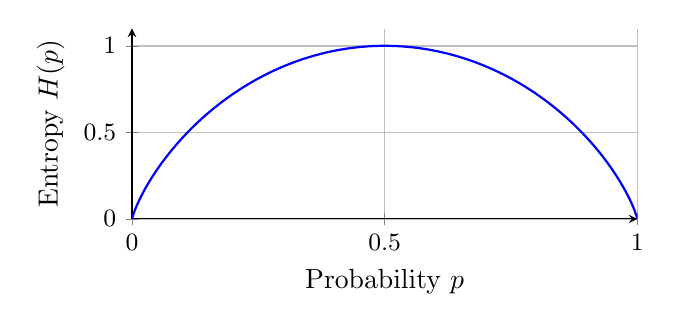
\begin{tikzpicture}
      \begin{axis}[
          width=8cm,
          height=4cm,
          xlabel={Probability \( p \)},
          ylabel={Entropy \( H(p) \)},
          ymin=0, ymax=1.1,
          xmin=0, xmax=1,
          ytick={0, 0.5, 1},
          xtick={0, 0.5, 1},
          domain=0:1,
          samples=200,
          grid=both,
          major grid style={line width=0.6pt, draw=gray!50},
          minor grid style={line width=0.3pt, draw=gray!30},
          tick label style={font=\small},
          axis lines=left
      ]
        \addplot[
          thick,
          blue,
        ]
        {-x*log2(x) - (1-x)*log2(1-x)} node[pos=0.5, above, sloped, xshift=-0.5cm, yshift=0.3cm] {};
      \end{axis}
    \end{tikzpicture}
    \caption{\label{fig:entropy_graph} Graph of entropy \( H(p) = -p \log_2(p) - (1-p) \log_2(1-p) \) for a fair coin toss.}
\end{figure}

\autoref{fig:entropy_graph} shows an example of the entropy in function of the probability of heads or tails when flipping a fair
coin.

\end{example}

\chapter{Randomness} \label{chap:randomness}

Compression, logically, can be interpreted as the removal of redundancy.
The compressed data therefore has no structure and cannot be distinguished from random data; in fact, it is random
(see \cite{AConciseIntroductionToDataCompression}).

\section{Origins}

Kolmogorov\footnote{Andrey Nikolaevich Kolmogorov (1903-1987) was a Soviet mathematician who played a central role in the creation
of modern probability theory. He also contributed to the mathematics of algorithmic information theory.} was one of first
mathematicians that wrote about randomness.

In 1964 and 1965, Martin-Löf\footnote{Per Erik Rutger Martin-Löf (born 1942) is a Swedish logician, philosopher, and mathematical
statistician.} was a student in Moscow under the supervision of Kolmogorov.
In 1966, he wrote "The definition of random sequences" that gave the first suitable definition of a random sequence.

Martin-Löf extended the definition for random elements with three approaches (from \cite{AlgorithmicRandomnessAndComplexity}) to
the definition of algorithmic randomness for infinite sequences:

\begin{definition}
The \textbf{computational paradigm}: Random sequences are those whose initial segments are all hard  to describe, or,
equivalently, hard to compress.
\end{definition}

\begin{definition}
The \textbf{measure-theoretic paradigm}: Random sequences  are those with no "effectively rare" properties.
If the class of sequences satisfying a given property is an effectively null set, then a random sequence should not have this
property.
This approach is the same as the stochastic paradigm: a random sequence should pass all effective statistical tests.
\end{definition}

\begin{definition}
The \textbf{unpredictability paradigm}: This approach stems from what is probably the most intuitive conception of randomness,
namely that one should not be able to predict the next bit of a random sequence, even if one knows all preceding bits, in the same
way that a coin toss is unpredictable even given the results of previous coin tosses.
\end{definition}

Despite the definitions the real innovation by Martin-Löf was the introduction of tests for randomness
(\cite{TheDefinitionOfRandomSequences}).

\begin{example}
Let's consider a long binary sequence \(000\dots0\) of all zeros.
It can be said that this sequence does not converge to \(1/2\) in the probability of 1 and 0, so it is clearly non-random.
But the reverse is not true: For instance \(101101101\dots101\) is not random because 101 occurs too often.
Moreover sequences that are not random like the digits of \(\pi\), cause the most difficulties.
In general, tests for randomness help us to understand if a sequence is random or not.
\end{example}

\section{Algorithmic Information Theory}

Following these studies the algorithmic information theory\footnote{The field of algorithmic information theory (AIT) arises by
mixing information theory and computation theory to obtain an objective and absolute notion of information in an individual
object.} (see \cite{AlgorithmicInformationTheoryBriefGuide}) formally defines what is randomness of individual objects
(binary strings).

\begin{definition}
\textbf{Kolmogorov complexity} of a binary sequence is the length of the shortest binary program that generates that sequence on a
universal Turing machine (\cite{ThreeApproachesToTheQuantitativeDefinitionOfInformation}).
\end{definition}

The concept essentially asserts that a binary sequence is considered random if there is no algorithm shorter than the sequence
itself that can generate it.
Another way to say it is that a binary sequence has no simple description other than writing down the string itself.

That is related to the concept of incompressibility in algorithmic randomness: a random sequence cannot be compressed into a
shorter representation than its original size.

So, loosely speaking, the randomness (or Kolmogorov complexity) of a finite sequence is equal to its shortest description.

Furthermore it is known that the Kolmogorov complexity is not computable.

\section{Random Sequences}

Randomness is a complex concept and it is not given for free in our devices.
The generation of random sequence is something that requires attention and must be handled with care.
A random sequence should satisfy three conditions:

\begin{itemize}
  \item The sequence follows a uniform distribution.
  \item Each element of the sequence is independent of each other.
  \item The rest of the sequence can not be predicted from any sequence.
\end{itemize}

Random numbers can be divided into two categories: true random numbers and pseudo-random numbers.
True random number generators (RNGs) are composed of two parts: entropy source and algorithm post-processing.
Pseudo random number generators (PRNGs) take a seed as input and generate an output sequence by function.

Nowadays, in commercial computers only PRNGs are available, in fact entropy sources are something external from digital computers.
In practice an entropy source is a physical or natural phenomenon that provides unpredictable, non-deterministic data.
Considering quantum computing\footnote{A quantum computer is a computer that exploits quantum mechanical phenomena. Here the bit
is replaced by the qubit, that in opposition to it has not two states but a probabilistic output of a classical bit.} the things
could be completely different.
In fact intrinsically random properties of quantum systems are one possible entropy source.

\chapter{Data Compression}

When discussing compression algorithms it is important to make a distinction between two components: the \textbf{model} and the
\textbf{coder}.
The model component somehow captures the probability distribution of the symbols (or messages) by knowing or discovering something
about the structure of the input.
The coder component then takes advantage of the probability knowledge acquired in the model to generate codes to represent the
symbols (or messages).
It does this by effectively lengthening low probability messages and shortening high-probability messages.
It should be pointed out that the line between model and coder components of algorithms is not always well defined, nevertheless
it is important to consider that modeling and coding are two distinctly different things.

\section{Techniques}

The compression techniques can be \textit{lossless} or \textit{lossy}.
The first category is the most theoretical, in fact it preserves data as they are.
Lossless compression ratios are generally in the range of 2:1 to 8:1.
Lossy compression, in contrast, works on the assumption that the data doesn't have to be stored perfectly.
Most information can be simply thrown away; the data will still be of acceptable quality.
This technique is frequently used in image and video compression, where a group of pixels can be approximated into a single value.
In this case the ratio can be of orders greater.
In conclusion lossless compression has a lower ratio because it preserves all information that can be reload back to the original
data, on the other hand, lossy compression has a bigger ratio but it discards some information and doesn't generate the same data
when it is reloaded.

\subsection{Modeling}

It can be statistical or dictionary-based.
Statistical modeling reads in and encodes a single symbol at a time using the probability of that character's appearance.
Dictionary-based modeling uses a single code to replace strings of symbols.
This techniques can be static or adaptive.
In the second case the problem of knowing the generated structure, the table of probabilities or the dictionary,
both when encoding and when decoding, is avoided.

\subsubsection{Statistical Modeling}

It uses a static table of probabilities.
At the beginning the model was created only the first time and then it is reused many times for different data.
The next enhancement was to build a statistics table for every unique input stream.
The number of symbols (usually characters) is called order of the model.
In particular order-N indicates that are considered N characters before the current one.
The order is important because it determines the size of the table.
The higher the order, the larger the table.
However, as the order increases, the algorithm's efficiency ratio also improves, up to the point where the overhead of
reading these tables becomes significant.
An alternative approach is to use adaptive models, that generates statistics while reading data.

\subsubsection{Dictionary Modeling}

It follows a different approach.
It reads in input data and looks for groups of symbols that appear in a dictionary.
It uses pointers to refer to groups of symbols at some point in the dictionary.
The longer the match, the better the compression ratio.
In this case the modeling is the core of the compression algorithm.
Also in this case the dictionary can be static or adaptive.

\subsection{Coding}

It generate codes to represent symbols or groups of symbols.

\subsection{Lossless Compression Techniques}

Lossless compression techniques are used to compress archives and files that need to be preserved as they are.
For details on the following implementations and their examples, see \cite{TheDataCompressionBook2ndEdition} and
\cite{IntroductionToDataCompression}.

\subsubsection{Morse Code (1837)}

It was based on the fact that shorter code should be assigned to the most frequent symbols used in English communication.

\begin{figure}[H]
  \centering
  \includegraphics[width=0.7\textwidth]{morse-code-characters-infographic}
  \caption{Table of the various Morse code characters}
  \label{fig:morse_code_pdf}
\end{figure}

In \autoref{fig:morse_code_pdf} it can be observed that the letter "e" which is the most commonly used letter in the English
language is assigned the symbol of a single dot.
The difference in the length of encoding different symbols can be considered as a need that explains why data compression is
important.
It takes the name from Morse\footnote{Samuel Finley Breese Morse (1791-1872) was an American inventor and painter. After
establishing his reputation as a portrait painter, Morse, in his middle age, contributed to the invention of a single-wire
telegraph system based on European telegraphs. He was a co-developer of Morse code in 1837 and helped to develop the commercial
use of telegraphy.}, a co-developer, that in 1837 helped to develop the commercial use of telegraphy.
For further information see
\url{https://www.electronics-notes.com/articles/summary-infographics/morse-code/morse-code-characters-infographic.php}.

\subsubsection{Shannon-Fano coding (1950)}

Shannon at Bell Labs and Fano\footnote{Roberto Mario "Robert" Fano (1917-2016) was an Italian-American computer scientist and
professor of electrical engineering and computer science at the Massachusetts Institute of Technology.} at MIT developed this
method nearly simultaneously\footnote{This method was proposed in Shannon's "A Mathematical Theory of Communication" (1948) and
in a later technical report by Fano (1949).}.
It is necessary to know the probability of each symbol's appearance in a message.
A table of codes could be constructed that has several important properties:

\begin{itemize}
  \item Different codes have different numbers of bits.
  \item Codes for symbols with low probabilities have more bits, and codes for symbols with high probabilities have fewer bits.
  \item Though the codes are of different bit lengths, they can be uniquely decoded.
\end{itemize}

Arranging the codes as a binary tree solves the problem of decoding these variable-length codes.

The actual algorithm is:

\begin{enumerate}
  \item For a given list of symbols, develop a corresponding list of probabilities or frequency counts so that each symbol's
  relative frequency of occurrence is known.
  \item Sort the lists of symbols according to frequency, with the most frequently occurring symbols at the top and the least
  common at the bottom.
  \item Divide the list into two parts, with the total frequency counts of the upper half being as close to the total of the
  bottom half as possible.
  \item The upper half of the list is assigned the binary digit 0, and the lower half is assigned the digit 1. This means
  that the codes for the symbols in the first half will all start with 0, and the codes in the second half will all start
  with 1.
  \item Recursively apply the steps 3 and 4 to each of the two halves, subdividing groups and adding bits to the codes
  until each symbol has become a corresponding code leaf on the tree.
\end{enumerate}

\begin{example}
In the following tables the execution steps of the algorithm are explained in a specific example
(taken from \cite{TheDataCompressionBook2ndEdition}).

The input data are:

\begin{table}[H]
  \begin{tblr}{
      colspec={*{2}{Q[l]}X[l]},
      row{odd}={gray!15},
      row{even}={white},
      row{1}={bg=gray!90,fg=white},
      colsep=4pt
    }
      \textbf{Symbol} & \textbf{Count} & \\
      \textbf{A} & 15 & \\
      \hline
      \textbf{B} & 7 & \\
      \hline
      \textbf{C} & 6 & \\
      \hline
      \textbf{D} & 6 & \\
      \hline
      \textbf{E} & 5 & \\
      \hline
  \end{tblr}
  \caption{\label{tab:ex_shannon-fano_input} Input data.}
\end{table}

\autoref{tab:ex_shannon-fano_input} shows data of a widespread example about minimum redundancy
coding\footnote{It is a code constructed in such a way that the average number of coding digits per message is minimized.}.

The result of the first step is:

\begin{table}[H]
  \begin{tblr}{
      colspec={*{3}{Q[l]}X[l]},
      width=\textwidth,
      row{odd}={gray!15},
      row{even}={white},
      row{1}={bg=gray!90,fg=white},
      colsep=4pt
    }
      \textbf{Symbol} & \textbf{Count} & & \\
      \textbf{A} & 15 & \textcolor{red}{0} & \\
      \textbf{B} & 7 & \textcolor{red}{0} & \\
      \cline[1.5pt,red]{1-3}
      % \cline{4-4}
      \textbf{C} & 6 & \textcolor{red}{1} & \\
      \textbf{D} & 6 & \textcolor{red}{1} & \\
      \textbf{E} & 5 & \textcolor{red}{1} & \\
      \hline
  \end{tblr}
  \caption{\label{tab:ex_shannon-fano_output1} Shannon-Fano output of the first step.}
\end{table}

\autoref{tab:ex_shannon-fano_output1} shows with a red line the split of the first step.

The result of the other steps is:

\setlength{\arrayrulewidth}{1.5pt}
\arrayrulecolor{red}

\begin{table}[H]
  \begin{tblr}{
      colspec={*{5}{Q[l]}X[l]},
      width=\textwidth,
      row{odd}={gray!15},
      row{even}={white},
      row{1}={bg=gray!90,fg=white},
      colsep=4pt
    }
      \textbf{Symbol} & \textbf{Count} & & \\
      \textbf{A} & 15 & \textcolor{red}{0} & \textcolor{red}{0} & \\
      \cline[1.5pt,red]{1-4}
      % \cline{5-6}
      \textbf{B} & 7  & \textcolor{red}{0} & \textcolor{red}{1} & \\
      \cline[1.5pt,red]{1-3}
      % \cline{4-6}
      \textbf{C} & 6  & \textcolor{red}{1} & \textcolor{red}{0} & \\
      \cline[1.5pt,red]{1-4}
      % \cline{5-6}
      \textbf{D} & 6  & \textcolor{red}{1} & \textcolor{red}{1} & \textcolor{red}{0} & \\
      \cline[1.5pt,red]{1-5}
      % \cline{6-6}
      \textbf{E} & 5  & \textcolor{red}{1} & \textcolor{red}{1} & \textcolor{red}{1} & \\
      \hline
  \end{tblr}
  \caption{\label{tab:ex_shannon-fano_output} Shannon-Fano final output.}
\end{table}

\autoref{tab:ex_shannon-fano_output} shows with horizontal red lines the Shannon-Fano steps by showing the splits.

Another view of the structure is:

\begin{figure}[H]
  \centering
    \begin{forest}
      for tree={
        draw, % Draw a box around each node
        circle, % Node shape (can be changed to rectangle, etc.)
        minimum size=1.5em, % Size of the node
        inner sep=2pt, % Space between text and node border
        l=1.5cm, % Level distance
        s sep+=1cm, % Sibling distance
        align=center % Enable multiline text in nodes
      }
      [
        [, edge label={node[midway,left]{0}}
          [\textbf{A}, edge label={node[midway,left]{0}}]
          [\textbf{B}, edge label={node[midway,right]{1}}]
        ]
        [24, edge label={node[midway,right]{1}}
          [\textbf{C}, edge label={node[midway,left]{0}}]
          [, edge label={node[midway,right]{1}}
            [\textbf{D}, edge label={node[midway,left]{0}}]
            [\textbf{E}, edge label={node[midway,right]{1}}]
          ]
        ]
      ]
    \end{forest}
    \caption{\label{fig:ex_shannon-fano_tree} Shannon-Fano tree.}
\end{figure}

\autoref{fig:ex_shannon-fano_tree} shows the Shannon-Fano binary tree.

The symbols with higher probability of occurrence (higher count) have fewer bits in their code.

The given results can be compared with some computations about the information theory.
In the following table .

\begin{table}[H]
  \begin{tblr}{
      colspec={*{6}{X[l]}},
      width=\textwidth,
      row{odd}={gray!15},
      row{even}={white},
      row{1}={bg=gray!90,fg=white},
      colsep=4pt
    }
      \textbf{Symbol} & \textbf{Count} & \textbf{Information} & \textbf{\hyperref[eq:information2]{Number of Bits}}
       & \textbf{SF Size} & \textbf{SF Bits} \\
      \textbf{A} & 15 & \hyperref[eq:information2]{1.38} & 20.68 & 2 & 30 \\
      \hline
      \textbf{B} & 7 & \hyperref[eq:information2]{2.48} & 17.35 & 2 & 14 \\
      \hline
      \textbf{C} & 6 & \hyperref[eq:information2]{2.70} & 16.20 & 2 & 12 \\
      \hline
      \textbf{D} & 6 & \hyperref[eq:information2]{2.70} & 16.20 & 3 & 18 \\
      \hline
      \textbf{E} & 5 & \hyperref[eq:information2]{2.96} & 14.82 & 3 & 15 \\
      \hline
  \end{tblr}
  \caption{\label{tab:ex_shannon-fano_information} Information for each symbol.}
\end{table}

\autoref{tab:ex_shannon-fano_information} shows the amount of \textbf{Information} that is computed with
\autoref{eq:information2}, while the \textbf{Number of Bits} is computed with \(count \cdot \autoref{eq:information2}\)

\end{example}

\subsubsection{Huffman coding (1952)}

It is similar to the Shannon-Fano coding. It was introduced two years later then the Shannon-Fano coding.
It was first published in 1952 by Huffman\footnote{David Albert Huffman (1925-1999) was an American pioneer in computer science,
known for his Huffman coding.} with a paper: "A Method for the Construction of Minimum Redundancy Codes".
It is more efficient than the other one.
The Shannon-Fano tree is built top-down, starting by assigning the most significant bits to each code and working down
the tree until finished.
Instead, Huffman codes are constructed bottom-up, beginning with the tree's leaves and progressing toward its root.

The tree is then built with the following steps:

\begin{itemize}
    \item The two free nodes with the lowest weights are located.
    \item A parent node for these two nodes is created. It is assigned a weight equal to the sum of the two child nodes.
    \item The parent node is added to the list of free nodes, and the two child nodes are removed from the list.
    \item One of the child nodes is designated as the path taken from the parent node when decoding a 0 bit.
    The other is arbitrarily set to the 1 bit.
    \item The previous steps are repeated until only one free node is left. This free node is designated the root of the tree.
\end{itemize}

\begin{example}

Reconsidering the \autoref{tab:ex_shannon-fano_input} input let's apply the Huffman coding algorithm.
The result is shown:

\begin{figure}[H]
  \centering
    \begin{forest}
      for tree={
        draw,
        circle,
        minimum size=1.5em,
        inner sep=2pt,
        l=1.5cm,
        s sep+=1cm,
        align=center
      }
      [39
        [{\textbf{A}\\15}, edge label={node[midway,left]{0}}]
        [24, edge label={node[midway,right]{1}}
          [13, edge label={node[midway,left]{0}}
            [{\textbf{B}\\7}, edge label={node[midway,left]{0}}]
            [{\textbf{C}\\6}, edge label={node[midway,right]{1}}]
          ]
          [11, edge label={node[midway,right]{1}}
            [{\textbf{D}\\6}, edge label={node[midway,left]{0}}]
            [{\textbf{E}\\5}, edge label={node[midway,right]{1}}]
          ]
        ]
      ]
    \end{forest}
    \caption{\label{fig:ex_huffman_tree} Huffman tree.}
\end{figure}

\autoref{fig:ex_huffman_tree} shows the Huffman binary tree, this can be compared with \autoref{fig:ex_shannon-fano_tree}.

The codes generated are:

\begin{table}[H]
  \begin{tblr}{
      colspec={*{2}{X[l]}},
      width=\textwidth,
      row{odd}={gray!15},
      row{even}={white},
      row{1}={bg=gray!90,fg=white},
      colsep=4pt
    }
      \textbf{Symbol} & \textbf{Code} & \\
      \textbf{A} & 0 \\
      \hline
      \textbf{B} & 100 \\
      \hline
      \textbf{C} & 101 \\
      \hline
      \textbf{D} & 110 \\
      \hline
      \textbf{E} & 111 \\
      \hline
  \end{tblr}
  \caption{\label{tab:ex_huffman_codes} The Huffman codes table.}
\end{table}

\autoref{tab:ex_huffman_codes} shows them.

A comparison between this example for Shannon-Fano and Huffman codes follows:

\begin{table}[H]
  \begin{tblr}{
      colspec={*{6}{X[l]}},
      width=\textwidth,
      row{odd}={gray!15},
      row{even}={white},
      row{1}={bg=gray!90,fg=white},
      colsep=4pt
    }
      \textbf{Symbol} & \textbf{Count} & \textbf{Shannon-Fano Code Length} & \textbf{Shannon-Fano Bits}
       & \textbf{Huffman Code Length} & \textbf{Huffman Bits} \\
      \textbf{A} & 15 & 2 & 30 & 1 & 15 \\
      \hline
      \textbf{B} & 7 & 2 & 14 & 3 & 21 \\
      \hline
      \textbf{C} & 6 & 2 & 12 & 3 & 18 \\
      \hline
      \textbf{D} & 6 & 3 & 18 & 3 & 18 \\
      \hline
      \textbf{E} & 5 & 3 & 15 & 3 & 15 \\
      \hline
  \end{tblr}
  \caption{\label{tab:ex_shannon-fano_huffman_comparision} Information for each symbol.}
\end{table}

\autoref{tab:ex_shannon-fano_huffman_comparision} shows that Huffman is better than Shannon-Fano because it uses less bits.
As a matter of fact, for a message with an information content of 85.25 bits, Shannon-Fano coding requires 89 bits, but Huffman
coding requires only 87.

\end{example}

\subsubsection{RLE (1960s)}

Run-length encoding algorithm stores consecutive occurrences of the same data value as a single occurrence of that data value and
a counter of the number of consecutive occurrences.
In some certain circumstances it can be very useful and efficient specially if combined with other techniques.
In 1983 RLE was patented by Hitachi\footnote{Hitachi, Ltd. is a Japanese multinational conglomerate founded in 1910 and
headquartered in Chiyoda, Tokyo.}.

\subsubsection{Arithmetic coding (1976)}

Basic algorithms for arithmetic coding were developed independently by Jorma J. Rissanen\footnote{Jorma Johannes Rissanen
(1932-2020) was an information theorist, known for originating the minimum description length (MDL) principle and practical
approaches to arithmetic coding for lossless data compression.}, at IBM Research, and by Richard C. Pasco, a Ph.D. student at
Stanford University; both were published in May 1976.

Huffman coding is a fixed-length coding method available and it is the best available.
Nevertheless Huffman codes have to be an integral number of bits long, and this can sometimes be a problem.
If the probability of a character is 1/3, for example, the optimum number of bits to code that character is around 1.6 bits.
Huffman coding has to assign either one or two bits to the code, and either choice leads to a longer compressed message than is
theoretically possible. In fact Huffman is a non optimal coding technique.

Arithmetic coding bypasses the idea of replacing an input symbol with a specific code.
It replaces a stream of input symbols with a single floating-point output number.

\begin{example}

The message "BILL GATES", for example, would have the following probability distribution:

\begin{table}[H]
  \begin{tblr}{
      colspec={*{3}{X[l]}},
      width=\textwidth,
      row{odd}={gray!15},
      row{even}={white},
      row{1}={bg=gray!90,fg=white},
      colsep=4pt
    }
      \textbf{Symbol} & \textbf{Probability} & \textbf{Range} \\
      \textbf{` '} & 1/10 & \(0 < r < 0.1\) \\
      \hline
      \textbf{A} & 1/10 & \(0.1 < r < 0.2\) \\
      \hline
      \textbf{B} & 1/10 & \(0.2 < r < 0.3\) \\
      \hline
      \textbf{E} & 1/10 & \(0.3 < r < 0.4\) \\
      \hline
      \textbf{G} & 1/10 & \(0.4 < r < 0.5\) \\
      \hline
      \textbf{I} & 1/10 & \(0.5 < r < 0.6\) \\
      \hline
      \textbf{L} & 2/10 & \(0.6 < r < 0.8\) \\
      \hline
      \textbf{S} & 1/10 & \(0.8 < r < 0.9\) \\
      \hline
      \textbf{T} & 1/10 & \(0.9 < r < 1\) \\
      \hline
  \end{tblr}
  \caption{\label{tab:ex_arithmetic_input} Input data.}
\end{table}

\autoref{tab:ex_arithmetic_input} shows input data, how the are sorted and their range of probability.

The Arithmetic encoding algorithm is:

\begin{lstlisting}[language=CStyle, caption={Arithmetic encoding algorithm.}, label={lst:ex_arithmetic_encoding}]
  low = 0.0;
  high = 1.0;
  while ((c = getc(input)) != EOF) {
    range = high - low;
    high = low + range * high_range(c);
    low = low + range * low_range(c);
  }
  output(low);
\end{lstlisting}

Following the encoding process shown in \autoref{lst:ex_arithmetic_encoding} brings to the following result:

\begin{table}[H]
  \begin{tblr}{
      colspec={*{3}{X[l]}},
      width=\textwidth,
      row{odd}={gray!15},
      row{even}={white},
      row{1}={bg=gray!90,fg=white},
      colsep=4pt
    }
      \textbf{Symbol} & \textbf{Low Value} & \textbf{High Value} \\
       & 0.0 & 1.0 \\
      \hline
      \textbf{B} & 0.2 & 0.3 \\
      \hline
      \textbf{I} & 0.25 & 0.26 \\
      \hline
      \textbf{L} & 0.256 & 0.258 \\
      \hline
      \textbf{L} & 0.2572 & 0.2576 \\
      \hline
      \textbf{` '} & 0.2572 & 0.25724 \\
      \hline
      \textbf{G} & 0.257216 & 0.25722 \\
      \hline
      \textbf{A} & 0.2572164 & 0.2572168 \\
      \hline
      \textbf{T} & 0.25721676 & 0.2572168 \\
      \hline
      \textbf{E} & 0.257216772 & 0.257216776 \\
      \hline
      \textbf{S} & 0.2572167752 & 0.2572167756 \\
      \hline
  \end{tblr}
  \caption{\label{tab:ex_arithmetic_encoding} Arithmetic encoding.}
\end{table}

So the final value 0.2572167752 (as shown in \autoref{tab:ex_arithmetic_encoding}), will uniquely encode "BILL GATES".

The Arithmetic coding decoding algorithm is:

\begin{lstlisting}[language=CStyle, caption={Arithmetic decoding algorithm.}, label={lst:ex_arithmetic_decoding}]
  number = input_code();
  for (;;) {
    symbol = find_symbol_straddling_this_range(number);
    putc(symbol);
    range = high_range(symbol) - low_range(symbol);
    number = number - low_range(symbol);
    number = number / range;
  }
\end{lstlisting}

Following the decoding process shown in \autoref{lst:ex_arithmetic_decoding} brings to the following result:

\begin{table}[H]
  \begin{tblr}{
    colspec={*{5}{X[l]}},
    width=\textwidth,
    row{odd}={gray!15},
    row{even}={white},
    row{1}={bg=gray!90,fg=white},
    colsep=4pt
  }
    \textbf{Encoded Number} & \textbf{Output Symbol} & \textbf{Low Value} & \textbf{High Value} & \textbf{Range} \\
    0.2572167752 & \textbf{B} & 0.2 & 0.3 & 0.1 \\
    \hline
    0.572167752 & \textbf{I} & 0.5 & 0.6 & 0.1 \\
    \hline
    0.72167752 & \textbf{L} & 0.6 & 0.8 & 0.2 \\
    \hline
    0.6083876 & \textbf{L}  & 0.6 & 0.8 & 0.2 \\
    \hline
    0.041938 & \textbf{` '} & 0.0 & 0.1 & 0.1 \\
    \hline
    0.41938 & \textbf{G} & 0.4 & 0.5 & 0.1 \\
    \hline
    0.1938 & \textbf{A} & 0.2 & 0.3 & 0.1 \\
    \hline
    0.938 & \textbf{T} & 0.9 & 1 & 0.1 \\
    \hline
    0.38 & \textbf{E} & 0.3 & 0.4 & 0.1 \\
    \hline
    0.8 & \textbf{S} & 0.8 & 0.9 & 0.1 \\
    \hline
    0 & & & & \\
    \hline
  \end{tblr}
  \caption{\label{tab:ex_arithmetic_decoding} Arithmetic decoding.}
\end{table}

In summary, the encoding process is simply one of narrowing the range of possible numbers with every new symbol.
The new range is proportional to the predefined probability attached to that symbol.
Decoding is the inverse procedure, in which the range is expanded in proportion to the probability of each symbol as it is
extracted (see \autoref{tab:ex_arithmetic_decoding}).

\end{example}

\paragraph{Practical Matters}

Encoding and decoding a stream of symbols using arithmetic coding at first glance seems completely impractical.
Particularly because floating point numbers have many limitations on digital computers.
As it turns out, arithmetic coding is best accomplished using integer math.
Floating point math is not required.

\subsubsection{LZ77 (1977)}

This algorithm was introduced by Lempel and Ziv in 1977 with the paper: "A Universal Algorithm for Sequential Data Compression"
as part of \textit{IEEE Transactions on Information Theory} journal.

LZ77 is revolutionary because that compression uses previously seen text as a dictionary.
It achieves compression by replacing variable-length strings in the input text with fixed-size pointers into the dictionary.

The main data structure in LZ77 is a text window, divided into two parts.
The first consists of a large block of recently decoded text.
The second, normally much smaller, is a look-ahead buffer.
The look-ahead buffer has characters read in from the input stream but not yet encoded.

The normal size of the text window is several thousand characters.
The look-ahead buffer is generally much smaller, maybe ten to one hundred characters.
The algorithm tries to match the contents of the look-ahead buffer to a string in the dictionary.

LZ77 encodes in sequences of tokens.
Each token consists of three items:

\begin{enumerate}
  \item An offset to a phrase in the text window.
  \item The length of the phrase.
  \item The first symbol in the look-ahead buffer that follows the phrase.
\end{enumerate}

A token is a tuple: \texttt{(offset, length, next symbol)}.

The decompression algorithm is very similar to the compression one.
It reads in a token, outputs the indicated phrase, outputs the following character, shifts, and repeats.
It maintains the window, but it does not work with string comparisons.

The dictionary is the text window, so it is adaptive.

\subsubsection{LZ78 (1978)}

This algorithm was introduced by Lempel and Ziv in 1978 with the paper: "Compression of Individual Sequences via Variable-Rate
Coding" as part of \textit{IEEE Transactions on Information Theory} journal.

LZ78 abandons the concept of a text window.
Under LZ78, the dictionary is a potentially unlimited list of previously seen phrases.
LZ78 also outputs a series of tokens with essentially the same meanings of LZ77.
Unlike LZ77, the phrase length is not passed since the decoder knows it.

This time token is a tuple: \texttt{(index, next symbol)}.
Here "index" takes the place of "offset" because of the different structure of the dictionary.

LZ78 adds that phrase to the dictionary.
After the phrase is added, it will be available to the encoder at any time in the future, not just for the next few thousand
characters.

Also in this case the decompression algorithm is very similar to the compression one.

This algorithm is "greedy", so it takes locally optimal decision optimal choice at each stage.
The problem is that in many cases, like in this one, a greedy strategy does not produce an optimal solution.

\begin{example}

Consider the following input text: "DAD DADA DADDY DADO...".

\begin{table}[H]
  \begin{tblr}{
      colspec={*{3}{Q[l]}X[l]},
      width=\textwidth,
      row{odd}={gray!15},
      row{even}={white},
      row{1}={bg=gray!90,fg=white},
      colsep=4pt
    }
      \textbf{Output Phrase} & \textbf{Output Character} & \textbf{Encoded String} & \\
      0 & D & D & \\
      \hline
      0 & A & A & \\
      \hline
      1 & ` ' & `D ' & \\
      \hline
      1 & A & DA & \\
      \hline
      4 & ` ' & `DA ' & \\
      \hline
      4 & D & DAD & \\
      \hline
      1 & Y & DY & \\
      \hline
      0 & ` ' & ` ' & \\
      \hline
      6 & O & DADO & \\
      \hline
  \end{tblr}
  \caption{\label{tab:ex_lz78} LZ78 encoding.}
\end{table}

In \autoref{tab:ex_lz78} each new phrase that was not seen before is also added to the dictionary that initially was empty.
Step by step the dictionary helps to reduce the volume of data.

\end{example}

The previous example makes clear that the decompression is done without giving the dictionary to the decompressor, because the
compression algorithm always outputs the phrase and character components of a code before it uses them.
This is very important because in this way the compressed data is not burdened with carrying a large dictionary.

\subsubsection{LZW (1984)}

Lempel-Ziv-Welch algorithm was published by Welch in 1984 as an improved implementation of the LZ78 algorithm published by Lempel
and Ziv in 1978.

Here the token is simply a value: \texttt{index}.

LZW is able to simplify the token because of the way it stores items on the dictionary.
A new entry to the dictionary is the concatenation of the matched pattern and the next character from the input stream.
The "next symbol" is always part of the new entry being added to the dictionary.

The decoder, upon receiving the index, retrieves the matched pattern and updates its dictionary concatenating the matched pattern
and the next inferred character. This means that the dictionary is maintained adaptive.

\subsubsection{BWT (1994)}

Burrows-Wheeler transform rearranges a character string into runs of similar characters.
It was invented by Michael Burrows\footnote{Michael Burrows (born 1963) is a British computer scientist and the creator of the
Burrows-Wheeler transform.} and David Wheeler\footnote{David John Wheeler (1927-2004) was a computer scientist and
professor of computer science at the University of Cambridge.} in 1994.

If the original string had several substrings that occurred often, then the transformed string will have several places where a
single character is repeated multiple times in a row.

\subsubsection{ANS (2014)}

Asymmetric numeral systems is a family of entropy encoding methods introduced by Jarek Duda\footnote{Jarosław Duda (born 1963),
also known as Jarek Duda, is a Polish computer scientist and an assistant professor at the Institute of Computer Science and
Computational Mathematics of the Jagiellonian University in Kraków. He is known as the inventor of asymmetric numeral systems
(ANS), a family of entropy encoding methods widely used in data compression.} and used in data compression since 2014 due to
improved performance compared to previous methods.
ANS combines the compression ratio of arithmetic coding with a processing cost similar to that of Huffman coding.
It's tabled variant, tANS, is achieved by constructing a finite-state machine.

\subsection{Lossy Compression Techniques}

Lossy compression techniques are used for multimedia data (audio, images and video) especially in applications such as streaming
media and internet telephony.
However, when quality does start degrading in a noticeable way, it is important to make sure it degrades in a way that is least
objectionable to the viewer.
The following descriptions are taken from \cite{IntroductionToDataCompression} and \cite{TheDataCompressionBook2ndEdition}.

\subsubsection{Transform Coding}

The idea of transform coding is to transform the input into a different form which can then either be compressed better.
This means that these are lossless transformations that doesn't actually perform compression.
The discrete cosine transform (DCT) is one of the most commonly used, another example is the discrete Fourier transform (DFT).

\subsubsection{Scalar Quantization}

A way to implement lossy compression is to take the set of possible messages \(S\) and reduce it to a smaller set \(S'\) by
mapping each element of \(S\) to an element in \(S'\).
Since the mapping used in quantization is many-to-one, it is irreversible and therefore lossy.
This general technique is called quantization.
When the mapping is linear it can be talked about \textit{uniform scalar quantization}.
When it is nonlinear it can be talked about \textit{nonuniform scalar quantization}.
In practice nonuniform scalar quantization is usually better.

\subsubsection{Vector Quantization}

Vector quantization maps a multidimensional space into a smaller set of messages \(S'\).
Vector quantization is typically implemented by selecting a set of representatives from the input space, and then mapping all
other points in the space to the closest representative.
Typically representatives are found using a clustering algorithm that finds some number of clusters of points in the data.
A representative is then chosen for each cluster by either selecting one of the points in the cluster or using some different
strategy that starts from these points and calculates the representative.
Vector quantization is most effective when the variables along the dimensions of the space are correlated.

\subsubsection{Wavelet Compression}

The fact that cosine and Fourier transforms are periodic functions can create problems when the input contains strong aperiodic
features.
A solution could be to break up the input in fixed-size blocks and transform each block in isolation.
An alternative approach is to use basis functions, called "wavelets", that could be applied to the entire image, without requiring
blocking.

To derive a suitable set of basis functions it starts from a single function, the "mother function".
Whereas cosine and Fourier repeats indefinitely, we want the wavelet mother function, to be contained within some local region,
and approach zero as we stray further away.
The family of basis functions are scaled and translated versions of this mother function.

\subsubsection{Fractal Compression}

The term "fractal" was first used by Mandelbrot\footnote{Benoit B. Mandelbrot (1924-2010) was a Polish-born French-American
mathematician and polymath with broad interests in the practical sciences. He is recognized for his contribution to the field of
fractal geometry.} to designate objects that are self-similar at different scales.
A well-known example is the Mandelbrot set, that is a complex image that can be computed by a simple program with a very short
formula.
The idea behind fractal compression is that if we wish to transmit a value, we could instead transmit a function or some functions
that iteratively converges on that value.
The functions are mappings from images to images.
It is enough that encoder and decoder have agreed in advance about the functions to use.
The function family we choose is a set of "collage functions", which map regions of an image to similar regions elsewhere in the
image, modified by scaling, rotation, translation, and other simple transforms.

\subsubsection{Model-Based Compression}

The idea here is to characterize the source data in terms of some strong underlying model.
Both sender and receiver share a large body of a priori knowledge contained in the model itself (e.g., the fact that faces have
two eyes and one nose).
Other information are transmitted with any given data set.
Model-based encoding has found applicability in such areas as computerized recognition of four-legged animals or facial
expressions.

\section{Comparison of Algorithms}

The following factors refer mainly to lossless data compression, in the lossy case it is more complicated (for example it should
be considered how good is the approximation).
Measurements have to be considered as averages in practice, because they are different for every single sample so their value is
an approximation.

\subsection{Compression Ratio}

An important factor when considering data compression is the "compression ratio". It is simply the sample size reduction factor
(look at \autoref{eq:factor_compression_ratio}).

\begin{equation} \label{eq:factor_compression_ratio}
  compression\ ratio = \frac{decompressed\ file\ size\ (SIZE)}{compressed\ file\ size\ (SIZE)}
\end{equation}

\subsection{Compression Speed}

It is important is specific use cases, usually when the network is involved (look at \autoref{eq:factor_decompression_speed}).

\begin{equation} \label{eq:factor_compression_speed}
  compression\ speed\ (SIZE / s) = \frac{decompressed\ file\ size\ (SIZE)}{compression\ time\ (s)}
\end{equation}

\subsection{Decompression Speed}

As the compression speed, it is important is specific use cases, usually when the network is involved (look at
\autoref{eq:factor_decompression_speed}).

\begin{equation} \label{eq:factor_decompression_speed}
  decompression\ speed\ (SIZE / s) = \frac{decompressed\ file\ size\ (SIZE)}{decompression\ time\ (s)}
\end{equation}

\subsection{CPU Usage}

The use can differ from \(100 \%\) (a single core) to \(N \times 100 \%\) (\(N\) cores), where \(N\) is the number of logical
cores of the CPU\footnote{A central processing unit (CPU), also called a central processor, main processor, or just processor, is
the most important processor in a given computer. It executes instructions of a computer program.}.
It has to be considered than even if a multi-threaded algorithm is generally faster than it's equivalent single-threaded
algorithm, the higher CPU usage is something that could be considered in the comparison of algorithms, depending on the needs.
In practical tests the percentage could be different from a multiple of \(100 \%\), for example an average of the total execution
could be considered.

In most cases every algorithm is implemented to work on the CPU only, because GPUs are expensive, besides their hardware is
needed.
If it could work on the GPU\footnote{A graphics processing unit (GPU) is a specialized electronic circuit initially designed for
digital image processing and to accelerate computer graphics. After their initial design, GPUs were found to be useful for
non-graphic calculations computing parallel programs very efficiently.} it should be specified and tests should consider that.
In fact their results should not be compared with other algorithms implementations that work on the CPU, because they would be,
in most cases, inevitably slower.

\subsection{Memory Usage}

How much RAM\footnote{Random-access memory (RAM) is a form of electronic computer memory that can be read and changed in any
order, typically used to store working data and machine code.} the implementation of the algorithm needs.
In many cases an average is enough.

\subsection{Time}

It could be simply considered the \hyperref[subsubsec:wall_time]{total elapsed time}, but a more accurate analysis can be done.

\subsubsection{User Time}
\label{subsubsec:user_time}

The amount of CPU time spent executing user-level code.
It does not include time spent in kernel mode (e.g., for system calls or I/O operations).

\subsubsection{System Time}
\label{subsubsec:system_time}

The amount of CPU time spent executing system-level code on behalf of the program (in kernel mode).
It includes time spent handling system calls (reading a file, memory allocation, networking...) and overhead for interacting with
hardware or operating system resources.

\subsubsection{Wall Time}
\label{subsubsec:wall_time}

The actual elapsed real-world time taken for the program to run from start to finish.
It is the sum of the \hyperref[subsubsec:user_time]{\textit{user time}} and the
\hyperref[subsubsec:system_time]{\textit{system time}}.

\subsection{Randomness Tests}

For what said in \autoref{chap:randomness}, an interesting way to understand the efficiency of compression algorithms is to
analyze the randomness of the output string of the compression algorithm.

This factor is not so indicative like the others but some articles talk about this.
In \cite{OnTheRandomnessOfCompressedData} it is stated that surprisingly it can occur that the best compression schemes do not
have the most random output.
This suggests that these schemes can be further improved.

\chapter{Compression Tools}

It is important to consider that compression tools are logically separated:

\begin{itemize}
  \item A file archiver combines several files into one file.
  \item A compression tool compresses and decompresses a single file.
\end{itemize}

These tools are often used in sequence to create compressed archives.
In some programs the two phases are hidden by the program itself.

\section{Archiving}

It combines several files into a single file with a size equivalent to the sum of each single file dimension.

\subsection{Unix}

According to the Unix philosophy the archiving process is separated from the compression process.
Unix known programs that aim to archiving only are \texttt{ar}, \texttt{cpio}, \texttt{tar} and \texttt{libarchive}.

\texttt{ar} was the original archiver, but has been largely replaced by \texttt{tar}.
\texttt{tar} derived from "tape archive" , as it was originally developed to write data to sequential I/O devices with no file
system of their own, such as devices that use magnetic tape.

In 2001, IEEE defined a new pax format which is basically tar with additional extended attributes.
The name "pax" is an acronym for portable archive exchange, but is also an allusion to the Latin word for "peace"; intended as a
peaceful unification of both \texttt{tar} and \texttt{cpio}.

\texttt{libarchive} is a free and open-source library, it's development was started in 2003.
It works on most Unix-like systems and Windows.

\subsection{Windows}

By default treats ZIP archive format that supports lossless data compression.
Native support was added as of the year 2000 in Windows ME.

One of the most common programs used in Windows is \texttt{7z} (7-Zip) that has its own archive format called 7z, but can read and
write several others, so it is widespread for compatibility.

\subsection{Mac OS X}

Apple has included built-in ZIP support in macOS 10.3 (via BOMArchiveHelper, now Archive Utility) and later.

\section{Compression}

A comparison between some of the following compression tools can be found online but it is important to stay updated.
About compression in Linux many articles can be found.
At \url{https://www.redpill-linpro.com/techblog/2024/12/18/compression-tool-test.html} different algorithms are tested with a
single large file.
Moreover at \url{https://www.baeldung.com/linux/compression-methods-comparison} a more accurate comparison that uses the
\href{https://github.com/MiloszKrajewski/SilesiaCorpus}{Silesia Corpus GitHub repository} as a collection of files used for
compression benchmarks.

The following compression programs are lossless.

\subsection{lz4}
\label{subsec:lz4}

It is focused on compression and decompression speed.
It belongs to the LZ77 family.
It is multi-threaded by default.

\subsection{compress}
\label{subsec:compress}

It is focused on compression and decompression speed.
It uses LZW.
It is not multi-threaded.

\subsection{gzip}
\label{subsec:gzip}

GNU zip is based on the DEFLATE algorithm.
DEFLATE is a combination of LZ77 and Huffman coding.
It is not multi-threaded.
\texttt{pigz} is the parallel version.

\subsection{bzip2}
\label{subsec:bzip2}

It is the successor of the \texttt{bzip} obsolete version.
It uses several layers of compression techniques, such as run-length encoding (RLE), Burrows-Wheeler transform (BWT),
move-to-front transform (MTF), and Huffman coding.
It is not multi-threaded.
\texttt{pbzip2} is the parallel version.

\subsection{bzip3}
\label{subsec:bzip3}

It is a modern implementation of bzip2 with enhancements.
It is not multi-threaded.

\subsection{lzma}
\label{subsec:lzma}

For compression/decompression the Lempel-Ziv-Markov chain algorithm (LZMA) is used.
This algorithm was introduced in 1998 and is based on LZ77.
It was developed by Igor Pavlov the author of 7-Zip.
It is not multi-threaded.

\subsection{xz}
\label{subsec:xz}

For compression/decompression LZMA2 is used, it is an improved version of the Lempel-Ziv-Markov chain algorithm (LZMA).
It is multi-threaded by default.

\subsection{zstd}
\label{subsec:zstd}

Zstandard is a lossless data compression algorithm developed by Yann Collet at Facebook.
Zstandard uses a dictionary windows (like LZ77) combined with fast entropy-coding.
It uses Huffman coding and finite-state entropy (FSE) (a version of ANS, tANS).
Zstd is the corresponding reference implementation in C, released as open-source software\footnote{the official implementation is
available at \url{https://github.com/facebook/zstd}.} in 2016.
It is multi-threaded by default.

\appendix

\chapter{Conclusions}

The distinction between data and information serves as the foundation for understanding data compression.

A brief introduction to information theory highlighted the origins of this discipline and its key principles.

The report demonstrated how information can be quantified and showed that "uncertainty" is measured as entropy.

Additionally, the concept of randomness and its relationship to data compression and algorithmic information theory was explored.
Generating truly random sequences in digital computers was shown to be a challenging task.

An overview of the most prominent lossless and lossy compression algorithms, along with the metrics used to evaluate them,
provided a basis for analyzing and comparing different compression tools.
A detailed comparison of lossless compression tools offered insight into the options currently available in the market.

The choice of a compression method ultimately depends on the specific requirements of the task at hand.

For tasks where speed is a priority, tools with a lower compression ratio, such as \hyperref[subsec:compress]{\texttt{compress}}
and \hyperref[subsec:lz4]{\texttt{lz4}}, are ideal.
For small files, fast compression tools like \hyperref[subsec:gzip]{\texttt{gzip}}, or its improved variant
\hyperref[subsec:gzip]{\texttt{pigz}}, are effective.
Large files benefit from high compression ratio tools such as \hyperref[subsec:bzip2]{\texttt{bzip2}}, or its improved variant
\hyperref[subsec:bzip2]{\texttt{pbzip2}}, and \hyperref[subsec:bzip3]{\texttt{bzip3}}.

The file type also plays a crucial role, textual data typically compresses well with the tools discussed earlier.
On the other hand binary files might see better results with \hyperref[subsec:zstd]{\texttt{zstd}} which has a high compression
ratio and impressive fast.
Lastly, tools like \hyperref[subsec:lzma]{\texttt{lzma}} and \hyperref[subsec:xz]{\texttt{xz}} deliver remarkable compression
levels but require significantly more time to process.

The final decision should balance the trade-offs between the compared parameters (compression speed, ratio...), and the specific
characteristics of the data being compressed.

\printbibliography
\thispagestyle{empty}

\end{document}
